\newpage{}
\begin{problem}{Multi Layer Perceptron (MLP) from Scratch \hfill {[20 pts]}}{prob:mlp}

At a high level, neural networks are functions $G_\theta: \mathbb{R}^n \rightarrow \mathbb{R}^m$. This notation means that $G$ is a function with parameters $\theta$, domain $\mathbb{R}^n$, and range $\mathbb{R}^m$. So $G$ takes in an input vector with $n$ \textit{features} and outputs a vector with $m$ \textit{features}. $G$ will be a very long expression with many different parameters, but since we'll compose it using only \verb|Value|'s, we can backpropagate and tune parameters exactly how we did in Problem 1 and 2. You will be writing a very tiny neural network library in \verb|grad/nn.py|, with a single type of model: the multi-layer perceptron (MLP). \\

\begin{figure}[H]
    \centering
    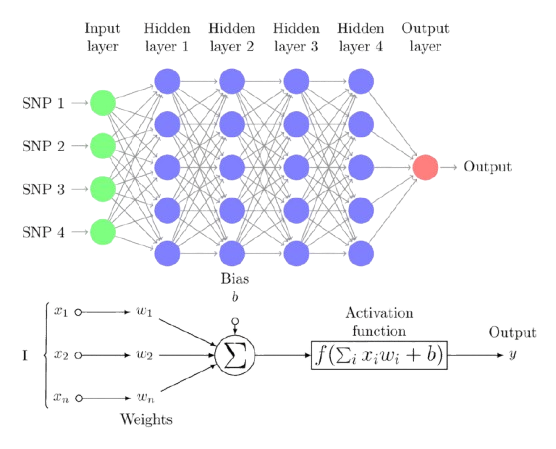
\includegraphics[width=0.75\linewidth]{media/mlp.png}
    \caption{}
    \label{fig:mlp}
\end{figure}

\vspace{10px}

\begin{adjustwidth}{2em}{2em}
    \textbf{(a)} Implement \verb|class Perceptron| \hfill (5 pts)\\
    \textbf{(b)} Implement \verb|class Layer| \hfill (5 pts)\\
    \textbf{(c)} Implement \verb|class MLP| \hfill (5 pts)\\
    \textbf{(d)} Train a PyTorch MLP on MNIST \hfill (5 pts)\\
    \begin{adjustwidth}{2em}{2em}
        \small
        Frameworks like PyTorch implement code for GPU/TPU accelerators 
        and make things faster by leveraging parallelism. At their core, however, they implement the same functionality as our scalar autograd engine. To make training feasible, you will use PyTorch's \verb|torch.nn| library, which exports an easy to use \verb|Linear| layer: \href{https://pytorch.org/docs/stable/generated/torch.nn.Linear.html}{read the docs here}. We've filled in some boilerplate, but left the model choice (how many layers, hyperparameters, learning rate, activation functions, biases, augmentation techniques, etc.) up to you.\\

        Train an MLP model that achieves 85\% classification accuracy on Fashion MNIST! Do not use convolution (that'll come in a later assignment). You are limited to MLP \verb|Linear| layers here. Please fill in all the TODO's in \verb|examples/ex_3d_fashion_pytorch.ipynb|.\\
        
        Include the final accuracy and loss vs. epochs plots in your submission.
    \end{adjustwidth}    
    
\end{adjustwidth}

\end{problem}

\begin{solution*}{}{}
    See code.

    \begin{center}
        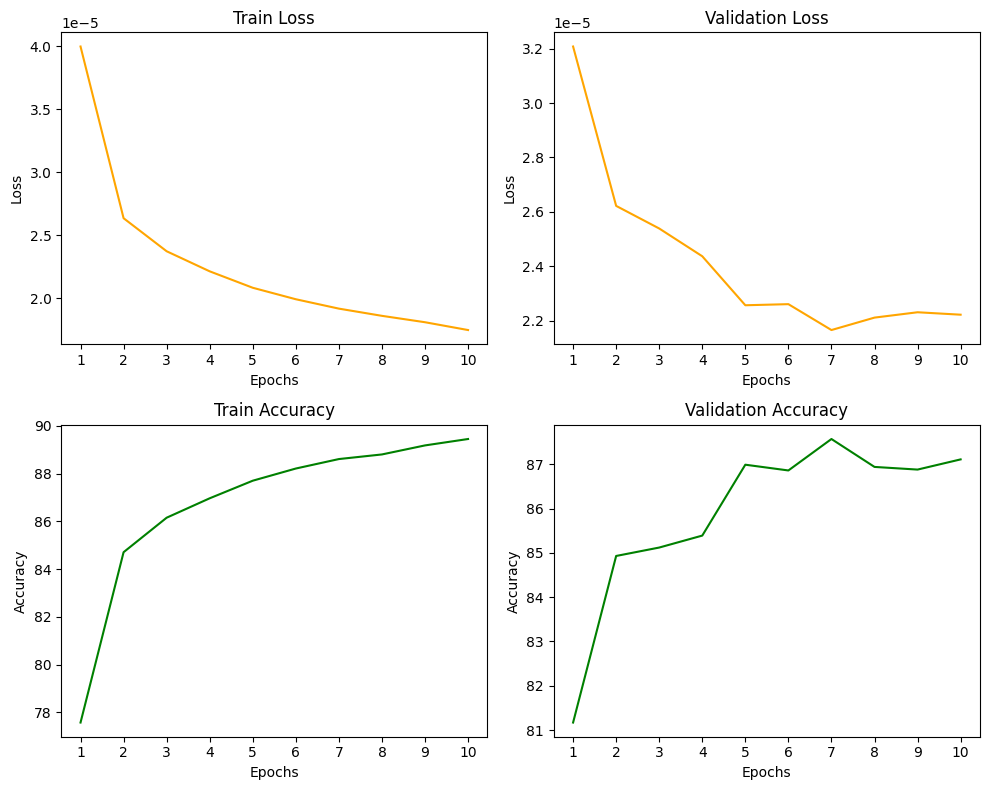
\includegraphics[width=\textwidth]{media/3.png}
    \end{center}
\end{solution*}
